\documentclass[border=0]{standalone}
\usepackage{booktabs}
\usepackage{tikz}

\usetikzlibrary{positioning}

\begin{document}
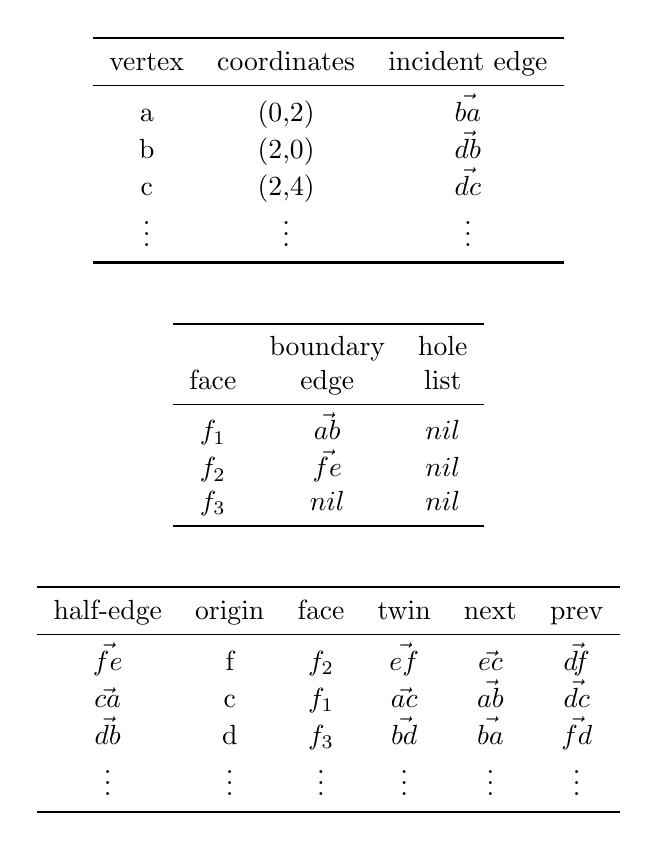
\begin{tikzpicture}
    \node[] (vertices) at (0,0) {
        \begin{tabular}{c c c}
                \toprule
                vertex & coordinates & incident edge \\
                \midrule
                a      & (0,2)  & $\vec{ba}$ \\
                b      & (2,0)  & $\vec{db}$ \\
                c      & (2,4)  & $\vec{dc}$ \\
                \vdots & \vdots & \vdots     \\
                \bottomrule
        \end{tabular}
    };
    \node[below = 5mm of vertices] (faces) {
        \begin{tabular}{c c c}
            \toprule
                & boundary  & hole\\
            face & edge      & list\\
            \midrule
            $f_1$ & $\vec{ab}$ & $nil$ \\
            $f_2$ & $\vec{fe}$ & $nil$ \\
            $f_3$ & $nil$      & $nil$ \\
            \bottomrule
        \end{tabular}
    };
    \node[below = 5mm of faces] (hedges) {
        \begin{tabular}{c c c c c c}
            \toprule
            half-edge & origin & face & twin & next & prev \\
            \midrule
            $\vec{fe}$ & f & $f_2$  & $\vec{ef}$ & $\vec{ec}$ & $\vec{df}$ \\
            $\vec{ca}$ & c & $f_1$  & $\vec{ac}$ & $\vec{ab}$ & $\vec{dc}$ \\
            $\vec{db}$ & d & $f_3$  & $\vec{bd}$ & $\vec{ba}$ & $\vec{fd}$ \\
            \vdots     & \vdots & \vdots & \vdots     & \vdots     & \vdots     \\
            \bottomrule
        \end{tabular}
    };

\end{tikzpicture}
\end{document}
